\documentclass{beamer}                             % presentation
% \documentclass[draft]{beamer}                    % improves compile time
% \documentclass[11pt, handout]{beamer}            % handout
\usepackage[utf8]{inputenc}                        % utf8
\usepackage[T1]{fontenc}                           % fix font encoding
\usepackage[english]{babel}                        % language
\usepackage{geometry, hyperref, fancyhdr, algorithm, multicol}
\usepackage{amsmath, amssymb, amsthm}              % ams mathematical packages
\usepackage{physics, mathtools, bm}                % extra math packages
\usepackage{graphicx, subcaption, wrapfig}         % images
\usepackage{fvextra, textcomp, CJKutf8}            % misc. text formatting
\usepackage[autostyle, english=american]{csquotes} % quotes
\usepackage{tikz, pgfplots, tikz-network}          % plots and graphs
\usepackage[noend]{algpseudocode}                  % algorithm psuedocode
\usepackage[cache=true]{minted}                    % source code
\usepackage[style=ieee]{biblatex}                  % bibliography

\pgfplotsset{compat=1.17}                          % version of pgfplots

\hypersetup{
  colorlinks=true,
  urlcolor=cyan,
  linkcolor=black
}

\setminted[]{
  linenos=false,
  breaklines=true,
  encoding=utf8,
  fontsize=\small,
  frame=lines,
  framesep=2mm
}

% https://tex.stackexchange.com/questions/343494/minted-red-box-around-greek-characters
\makeatletter
\AtBeginEnvironment{minted}{\dontdofcolorbox}
\def\dontdofcolorbox{\renewcommand\fcolorbox[4][]{##4}}
\makeatother

\graphicspath{{./images/}}
\addbibresource{ref.bib}

\newcommand{\emphasis}[1]{\textbf{\textit{#1}}}
\DeclareMathOperator*{\argmin}{argmin}
\DeclarePairedDelimiter\floor{\lfloor}{\rfloor}
\DeclarePairedDelimiter\ceil{\lceil}{\rceil}

\usetheme{Berkeley}
\usecolortheme{dolphin}
% hide navigation buttons
\setbeamertemplate{navigation symbols}{}

% title page
\title[]{\textit{k}-means, kd-Trees, and Median of Medians}
\subtitle{Color Quantization done fast}
\author[Huan]{Stephen Huan\inst{1}}
\institute[TJHSST]
{
  \inst{1}
  Thomas Jefferson High School for Science and Technology
}
\date[]{TJ Vision \& Graphics Club, December 2, 2020}
\subject{Computer Science}

\AtBeginSubsection[]
{
  \begin{frame}
    \frametitle{Table of Contents}
    \tableofcontents[currentsection, currentsubsection]
  \end{frame}
}

\begin{document}
\frame{\titlepage}

\section{Color Quantization}

\begin{frame}
\frametitle{Table of Contents}
\tableofcontents[currentsection]
\end{frame}

\begin{frame}
\frametitle{Color Quantization}
\framesubtitle{Reducing the number of colors}
\begin{columns}
\column{0.5\textwidth}
\uncover<1-> {
  \alert{Color quantization} is the process of reducing
  the number of colors in an image.
}

\uncover<2-> {
  For example, a typical RGB image stores 1 byte per color,
  so 24 bits over 3 colors.
}

\uncover<3-> {
  This has applications in compression, but is most often used for legacy
  hardware (whose memory is limited,
  so the number of bits/pixel must be limited).
}

\column{0.5\textwidth}
\uncover<1->{
  \begin{exampleblock}{An image amenable to color quantization} 
    \begin{figure}[h!]
      \centering
      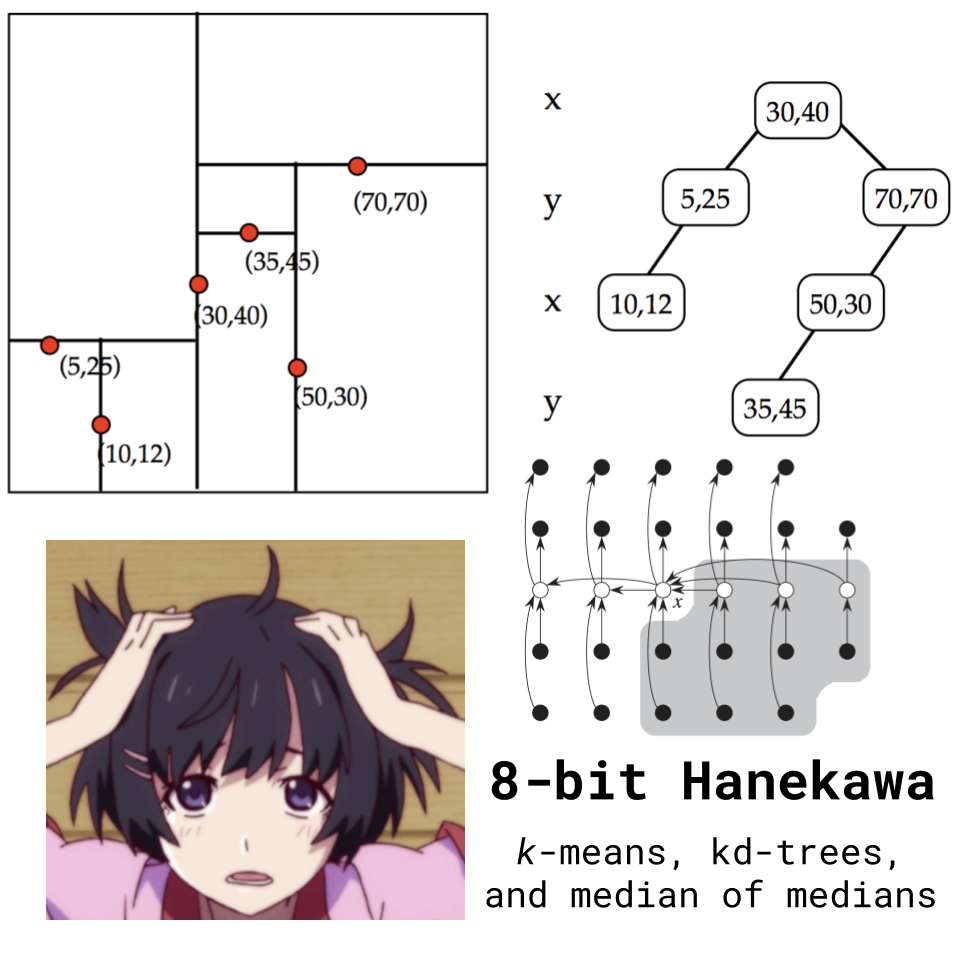
\includegraphics[scale=0.15]{cover_image.png}
      \caption{A summary of this lecture}
    \end{figure}
  \end{exampleblock}
}
\end{columns}
\end{frame}

\begin{frame}
\frametitle{Techniques}
\framesubtitle{}
Suppose we want to decompose an image into \( k \) distinct colors. \pause

One simple approach would be to find the \( k \)
most frequent colors and use those. \pause

This has a pretty obvious failure mode. \pause

\begin{exampleblock}{Failure mode for the frequency heuristic}
  Suppose we have an image with 4 colors: dark red has 50 pixels, light red
  has 49, dark blue has 48, and light blue has 47. If \( k = 2 \), then we 
  would choose dark red and light red, which would be problematic for the blues.
  A better selection would probably be to pick a normal red and a normal blue,
  at the cost of not showing the dark/light contrast within the colors.
\end{exampleblock}
\end{frame}

\begin{frame}
\frametitle{Techniques, continued}
\framesubtitle{}
We could address this by splitting our color space into color ranges, or using
a different algorithm like the \textit{median cut} algorithm, which constructs
a kd-tree on the color space. \pause

Today, we will discuss applying the  \textit{k}-means clustering technique
(an AI/ML lab here at TJ).
\end{frame}

\section{\textit{k}-means clustering}
\subsection{\textit{k}-means}
\begin{frame}
\frametitle{\textit{k}-means}
\framesubtitle{}
Suppose we have a set of points and a set of \( k \) \alert{center} points.
Define the \alert{Euclidean distance} between two points
as the magnitude of the vector difference, i.e.
\[ \texttt{dist}(\vec{u}, \vec{v}) = \norm{\vec{u} - \vec{v}}
= \sqrt{(u_1 - v_1)^2 + (u_2 - v_2)^2 + \dots} \] \pause 

We want to pick our center points such that they minimize the sum of the
distance between each point to its closest center, i.e.
\[ \argmin_{\text{centers}}
  \underbrace{\sum_{\vec{p} \in \text{points}}}_{\text{sum over all points}}
  \underbrace{\min_{\vec{c} \in \text{centers}} \texttt{dist}(\vec{p}, \vec{c})}_
{\text{closest center to \( \vec{p} \)}} \]
\end{frame}

\begin{frame}
\frametitle{\textit{k}-means, continued}
\framesubtitle{}
This problem is NP-hard, necessitating a greedy algorithm. \pause

\begin{block}{\textit{k}-means algorithm}
The standard algorithm alternates between two steps until convergence:
Given \textit{k} initial center points,
\begin{enumerate}[<+->]
  \item Assign each point to its closest center
  \item Update each center to the \alert{centroid} of the points assigned to it,
    where the centroid is the arithmetic mean.
\end{enumerate}

\end{block}

Intuitively, if the center points are fixed, then the best possible assignment
is to assign each point to its closest center. \pause
In the dual case, if the assignment of points to centers is fixed,
then the best possible center position is the mean point, i.e.
\[ E[S] = \frac{1}{\norm{S}} \sum_{\vec{p} \in S} \vec{p}  \]
\end{frame}

\begin{frame}
\frametitle{\textit{k}-means, continued}
\framesubtitle{}
\enquote{Convergence} is when after the centers are updated,
the assignment of points to their closest center 
is the same as the assignment before the update.
(the next center update would be the same). \pause

This finds a local optimum, not necessarily the global optimum. \pause

The number of iterations until convergence is also superpolynomial
in the worst case, but in general works quite well in practice.

Our pick for the initial \textit{k} centers is quite important!
\end{frame}

\subsection{\textit{k}-means++}

\begin{frame}
\frametitle{\textit{k}-means++}
\framesubtitle{An initialization scheme for \textit{k}-means}
\begin{block}{Two theoretical problems with \textit{k}-means}
  \begin{enumerate}
  \item Running time is superpolynomial with respect to the number of points
  \item Approximation can be made arbitrarily bad compared to the 
    optimal clustering \pause
\end{enumerate}
\end{block}

\textit{k}-means++ fixes the latter problem, it guarantees an \( O(\log k) \) 
approximation bound in expectation (i.e., over expectation the clusters
generated by \textit{k}-means++ has a distance of at most \( O(\log k) \)
times greater than the optimal cluster). \pause

How does it work?
\end{frame}

\begin{frame}
\frametitle{\textit{k}-means++, continued}
\framesubtitle{}
\begin{block}{\textit{k}-means++ algorithm}
  \begin{enumerate}
    \item Pick the first center point at random \pause
    \item From there, pick the next center point by sampling the probability
      distribution where a point \( \vec{p} \) is picked with weighting
      \( \texttt{dist}(\vec{p}, \vec{c})^2 \),
      where \( \vec{c} \) is the closest center \pause
    \item Repeat until \( k \) centers are picked
    \item Run \textit{k}-means as usual \pause
  \end{enumerate}
\end{block}
Intuitively, picking centers far away from each other is a good thing, so the
weighting favors points that are far away from the existing centers. \pause

Also, it's impossible to have two identical centers, since the distance of a
point to itself is 0, so its weighting would be 0. \pause

How do we sample this probability distribution?
\end{frame}

\begin{frame}[fragile]
\frametitle{Sampling a random variable}
\framesubtitle{}
\begin{algorithm}[H]
  \caption{Sampling a random variable}
  \begin{minted}[frame=none]{python}
    def sample(p: list) -> float:
        """ Samples a value from a random variable. """
        r = random.random()
        i = cmf = 0
        while i < len(p) - 1:
            cmf += p[i]
            if r < cmf:
                break
            i += 1
        return i
  \end{minted}
\end{algorithm}
\end{frame}

\begin{frame}
\frametitle{Sampling a random variable, justification}
\framesubtitle{}
Claim: This function has the same \textit{cumulative mass function}
as the underlying probability distribution. \pause

For a uniform random variable \( X \sim [0, 1] \), the probability that
\( X \) is less than some value \( x \), \( p(X \leq x) \), is 
\[ \int^{x}_0 1 \ dt = x \] \pause

The chance \texttt{sample} outputs an index \( \leq j \) is if the sum
of the probabilities up to \( j \) is greater than the uniform r.v. \( X \),
or flipping the inequality, if \( X \) is less than the sum. 
\[p(\texttt{sample} \leq j) =
p(X \leq \sum^{j}_{i = 0} p[i]) = \sum^{j}_{i = 0} p[i] \]  \pause
\end{frame}

\begin{frame}[fragile]
\frametitle{Sampling a random variable, continued}
\framesubtitle{}
By definition, this is the cmf of the discrete r.v. \pause

If \texttt{sample} has the same cmf as \( p \), then it has the same pmf.
If it has the same pmf, then this is "sampling the probability distribution"
represented by p by definition! \pause

\begin{block}{Step 2 of \textit{k}-means++, in detail} 
  \begin{enumerate}
    \item Make a list of the squared distances
      from a point to its nearest center.
    \item Normalize this list into a probability distribution
      by dividing by its sum: \mintinline{python}{p = [x/sum(l) for x in l]}
    \item Call \texttt{sample} to get a index which corresponds to a point.
    \item Add this point to the list of centers.
  \end{enumerate}
\end{block}
\end{frame}

\begin{frame}
\frametitle{Notes on \textit{k}-means++}
\framesubtitle{}
Yes, \textit{k}-means++ adds an additional \( k \) passes over the data
compared to picking \( k \) points at random. \pause

First, as stated earlier \textit{k}-means++ bounds the amount of error and will
generally produce higher quality clusters. \pause

Second, the better initialization also reduces the number of iterations until
convergence for \textit{k}-means, making it actually faster in practice.
\end{frame}

\begin{frame}
\frametitle{Notes on \textit{k}-means for color quantization}
\framesubtitle{}
Let's go back to the original problem, color quantization.
How do we apply \textit{k}-means for color quantization? \pause

If we want to reduce an image to \( k \) colors, we simply run \textit{k}-means,
where our points are the RGB values. This finds \( k \) colors,
and we assign each color in the original image
to the closest color in our \( k \) colors as usual, except we need to round
our \( k \) centers to integer pixel values. \pause 

Note 1: Euclidean distance is not the best in terms of
color difference perception (a smaller Euclidean distance does not necessarily
imply that the colors look closer compared to a larger distance).
We can change to the Lab color space or change distance measures.
\end{frame}

\begin{frame}
\frametitle{Notes on \textit{k}-means for color quantization, continued}
\framesubtitle{}
Note 2: Square roots are expensive, and if we don't ever need the
actual distance, we can always compute distance squared. \pause

We use \texttt{dist} in two ways:
\begin{enumerate}
  \item To find the closest center point to a given point
  \item To weight the probability distribution in \textit{k}-means++
\end{enumerate} \pause 

\( f(x) = x^2 \) is a \textit{monotonic} function,
i.e. if \( x < y \) then \( f(x) < f(y) \) (if \( x \) is nonnegative,
and distances are always nonnegative by definition).
Therefore, minimizing \( f(x) \) is equivalent to  minimizing \( x \).
The same trick is frequently used in machine learning loss functions. \pause

For use case 2, we weight a point by its squared distance.

Thus, what I call \enquote{\texttt{dist}} is in fact
\[ \texttt{dist}(\vec{u}, \vec{v}) = \norm{\vec{u} - \vec{v}}^2
= (u_1 - v_1)^2 + (u_2 - v_2)^2 + \dots \]
\end{frame}

\subsection{Practical Example}

\begin{frame}
\frametitle{Pokémon profile picture month}
\framesubtitle{}
As per TJ tradition, December is for \enquote{Pokémon profile pictures},
where people update their Facebook profile pictures (\enquote{pfp}'s)
to their favorite Pokémon.

\begin{figure}[h!]
    \centering
    \begin{subfigure}[h]{0.3 \textwidth}
      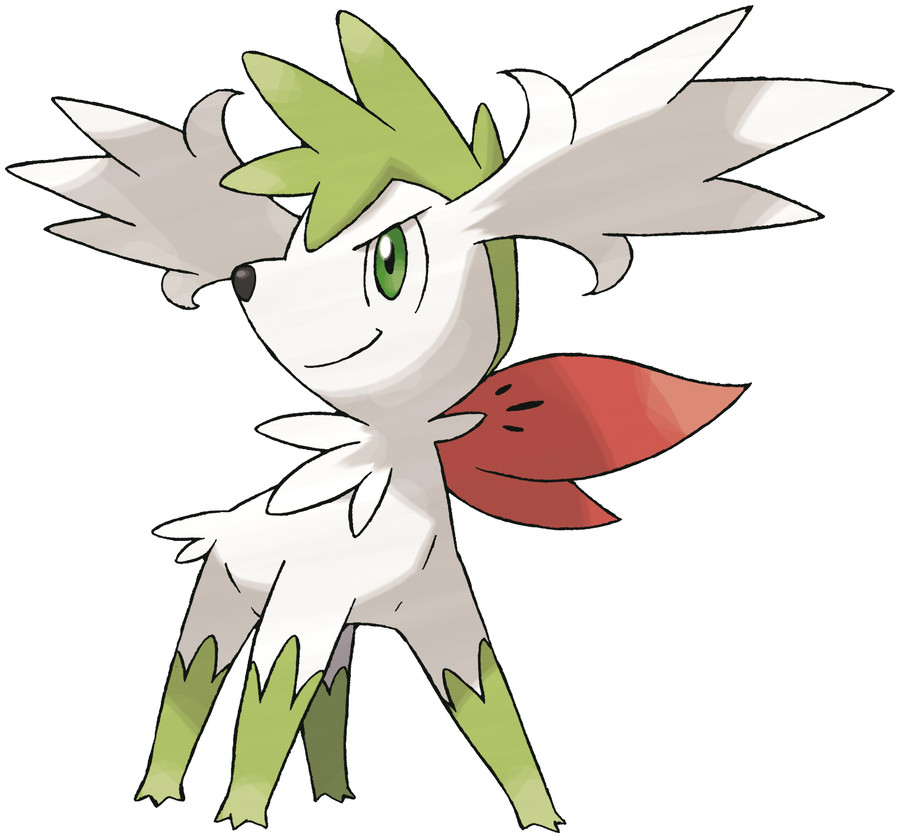
\includegraphics[scale=0.1]{shaymin-sky.jpg}
      \caption{The image I like, original Shaymin}
    \end{subfigure}
    \hfill
    \begin{subfigure}[h]{0.3 \textwidth}
      
\includegraphics[scale=1.17]{shaymin-color.png}
      \caption{The color scheme of a shiny Shaymin}
    \end{subfigure}
    \hfill
    \begin{subfigure}[h]{0.3 \textwidth}
      
\includegraphics[scale=0.1]{shaymin.png}
      \caption{First image with the second's color}
    \end{subfigure}
    \caption{Color transfer}
\end{figure}

Suppose I like the pose of the first image, but I want the Shaymin to be shiny.
Can I use \textit{k}-means to transfer the color?
\end{frame}

\begin{frame}
\frametitle{\textit{k}-means for Pokémon pfp month}
\framesubtitle{}

\begin{enumerate}
  \item Pick a good value of \( k \). \( k \) should be large enough such that
    the image still looks reasonably good, but small enough for you to be able
    to modify colors by hand. In this case, \( k = 16 \).
  \item Run \textit{k}-means as usual
  \item Identify which colors are green (to substitute with the shiny colors) 
  \item Temporarily set a green color to (0, 0, 255),
    i.e. an indicator color to see where it appears in the image.
  \item Identify the corresponding color in the shiny form
  \item Make the replacement 
\end{enumerate}
\end{frame}

\begin{frame}[fragile]
\frametitle{\textit{k}-means for Pokémon pfp month, code}
\framesubtitle{}
\begin{minted}[label=color modification]{python}
    centers, ids, groups = k_means(K, data)
    px = [tuple(round(c) for c in center) \
          for center in centers]
    # color modifications to make shiny
    px[ 5] = ( 55, 199, 179) # main color
    px[ 6] = ( 17, 112, 106) # eye color 
    px[ 8] = ( 97, 210, 182) # tips of head/feet
    px[15] = ( 35, 138, 123) # parts in shadow
\end{minted}
\end{frame}

\begin{frame}
\frametitle{Making \textit{k}-means faster}
\framesubtitle{}

Back to theory. If \textit{k}-means takes \( I \) iterations to converge
and there are \( N \) points, then the computational complexity is \( O(NKI) \)
as on each iteration, we need to compute the closest center to a point,
and the easiest way to do that is to iterate over each center point. There
are \( N \) points and \( K \) center points, so it takes \( O(NK) \). \pause

We can speed this up if we can compute the closest center point quicker,
which we can do with \alert{kd-trees}. 

\end{frame}

\section{kd-Trees}
\subsection{Construction}

\begin{frame}
\frametitle{kd-Tree}
\framesubtitle{}
\begin{block}{kd-tree}
  A kd-tree is essentially a binary search tree (BST) generalized to multiple
  dimensions. Each node has at most 2 children.
\end{block}
In a BST, to insert a value we compare it against the root's value, if it's less
we recur on the left subtree, if greater on the right subtree. \pause

A kd-tree is similar except each node holds a \textit{point}, not a value.
This point has \( D \) dimensions, and at each layer of the kd-tree we compare
against a particular \enquote{cutting dimension} \( d \). \pause

We typically cycle through cutting dimensions. 
\end{frame}

\begin{frame}
\frametitle{kd-Tree insert}
\framesubtitle{}

\begin{figure}[h!]
  \centering
  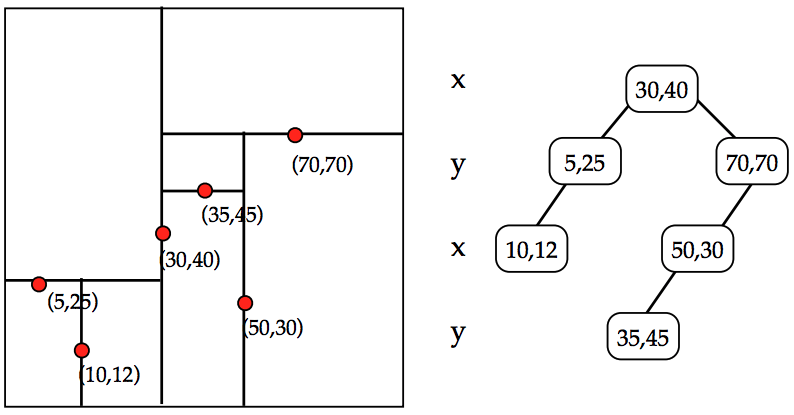
\includegraphics[scale=0.35]{kd-tree}
  \caption{kd-Tree in 2 dimensions}
\end{figure}
\end{frame}

\begin{frame}[fragile]
\frametitle{kd-Tree node}
\framesubtitle{}
\begin{minted}[label=kd-tree node]{python}
  class kdNode:

      def __init__(self, point: tuple=None, cd: int=0):
          self.child = [None, None]
          self.point = point
          self.D = len(point)
          self.cd = cd
\end{minted}

\begin{minted}[label=get children]{python}
    def dir(self, p: tuple) -> int:
        """ Gets the proper left/right child
            depending on the point p. """
        return p[self.cd] >= self.point[self.cd]
\end{minted}
\end{frame}

\begin{frame}[fragile]
\frametitle{kd-Tree insert code}
\framesubtitle{}
\begin{algorithm}[H]
  \caption{kd-Tree Insert}
  \begin{minted}[frame=none]{python}
    def __add(self, t, p: tuple, parent=None):
        if t is None:      # found leaf
            t = kdNode(p, (parent.cd + 1) % parent.D)
        elif t.point == p: # ignore duplicates
            return t
        else:              # update pointers
            t.child[t.dir(p)] = \
            self.__add(t.child[t.dir(p)], p, t)
        return t

    def add(self, p: tuple) -> None:
        # empty tree, simply change our own point
        if self.point is None:
            self.__init__(p)
        self.__add(self, p)
  \end{minted}
\end{algorithm}
\end{frame}

\begin{frame}
\frametitle{Runtime Analysis}
\framesubtitle{}
Like a BST, we would expect insert to take \( O(\log n) \), since we do a path
from root to leaf and in a balanced tree the depth is \( \log n \), where
\( n \) is the number of nodes (equivalent to the number of points). \pause 

However, there is a clear degenerate case: if each point increases along every
dimension, then the tree becomes a line with height \( O(n) \).
\( 1 + 2 + \dots + n = O(n^2) \), so it might take quadratic time to build
a kd-tree in the worst case. \pause

Common BST tricks like AVL trees seem difficult (are rotations even possible
if they change the cutting dimension?). \pause 

In practice, the points are commonly known ahead of time. Can we guarantee
an \( O(n \log n) \) build over \( n \) points if we know the \( n \) points
ahead of time?
\end{frame}

\subsection{Median-based Construction}

\begin{frame}
\frametitle{Pre-sort algorithm}
\framesubtitle{}
Observation: Splitting the points perfectly in half between the left and right
subtrees is the best possible split. Obviously, we split the points in half
based off the \textit{median} value. \pause

To efficiently keep track of the median, we make \( D \) copies of the \( N \)
points. We sort each copy on a different dimension. \pause

Finally, we pass this list of lists to the kd-Tree build function,
find the median point, split our list of lists into a left and right side,
and recursively build the tree. As long as we maintain the sorted invariant,
we can compute the median point on any dimension in \( O(1) \).
\end{frame}

\begin{frame}[fragile]
\frametitle{Pre-sort algorithm, code}
\framesubtitle{}
\begin{minted}[label=wrapper over kdNode]{python}
    class kdTreeSort(kdNode):

        def __init__(self, points: list=[]) -> None:
            super().__init__()
            if len(points) > 0:
                D = len(points[0])
                # no need for duplicate points
                self.points = list(set(points))
                # sort points on each dimension
                pointsd = [sorted(self.points,
                           key=lambda p: p[d])
                           for d in range(D)]
                build_tree(self, pointsd)
\end{minted}
\end{frame}

\begin{frame}[fragile]
\frametitle{Pre-sort algorithm, code}
\framesubtitle{}
\begin{minted}[label=split]{python}
    def subsplit(pointsd: list, seen: set) -> list:
        """ Only takes the points that are in seen. """
        return [[p for p in points if p in seen]
                for points in pointsd]

    def split(pointsd: list, cd: int, p: int) -> tuple:
        """ Splits by the plane x_cd = p[cd]. """
        left, right = set(), set()
        for point in pointsd[0]:
            if point != p:
                # add point with the same value as p
                # at cd to the right side
                (left if point[cd] < p[cd] \
                 else right).add(point)
        return subsplit(pointsd, left), \
               subsplit(pointsd, right)
\end{minted}
\end{frame}

\begin{frame}[fragile]
\frametitle{Pre-sort algorithm, code}
\framesubtitle{}
\begin{algorithm}[H]
  \caption{Pre-sort algorithm for kd-tree construction}
  \begin{minted}[frame=none,fontsize=\footnotesize]{python}
    def build_tree(t: kdNode, pointsd: list,
                   cd: int=0) -> kdNode:
        N, D = len(pointsd[cd]), len(pointsd)
        t.D, t.cd = D, cd
        t.point = pointsd[cd][N//2] # median
        next_cd = (cd + 1) % D
        t.child = [build_tree(kdNode(), l, next_cd) \
                   if len(l[0]) > 0 else None
                   for l in splitd(pointsd, cd, t.point)]
        return t
  \end{minted}
\end{algorithm}
\end{frame}

\begin{frame}
\frametitle{Runtime Analysis}
\framesubtitle{}
The running time is dominated by \texttt{subsplit}, which must split the \( D \)
copies of \( N \) points. Determining whether a point is in the left or right
set is at least an \( O(D) \) operation since the hash needs to take into
account each value of the point. There are \( O(ND) \) checks,
so \texttt{subsplit} runs in \( O(D^2 N) \).
Over the \( \log N \) levels of the tree, the pre-sort algorithm runs in
\( O(D^2 N \log N) \) (each level of the tree must split \( N \) points). \pause

We can improve \texttt{subsplit}'s performance by noticing that we don't
actually need to copy the points with all their dimensions; we can assign
an arbitrary distinct ID to each point and maintain the \( D \) lists
based off this integer ID. The simplest ID to use is the point's index
in the points list, as to go from an ID to a point is just indexing the list.
Since we only need the point values when comparing to the cutting dimension,
we can find the cutting dimension in \( O(1) \) by looking up the point and then
indexing the point at that cutting dimension.
\end{frame}

\begin{frame}
\frametitle{Runtime Analysis, continued}
\framesubtitle{}
This optimization shaves off a \( D \) factor, so our running time goes from
\( O(D^2 N \log N) \) to \( O(D N \log N) \) where the running time
is dominated by the \( D \) initial \( O(N \log N) \) sorts. \pause

Recall that we need to do the sorts to find the median efficiently. Can we
shave off another \( D \) factor if we find the median a different way? \pause

We could maintain a single list of points, and simply sort this list on the
cutting dimension at each level. That adds a \( \log N \) factor at every level,
so the running time is \( O(N \log^2 N) \). \pause

We could also just pick a random point to split on. This is equivalent to just
calling \texttt{add} repeatedly on each point, so it has the same quadratic
worst case running time. \pause

Luckily, there is a way to find the median of a list in linear time!
\end{frame}

\section{Finding Medians}
\subsection{Select}

\begin{frame}
\frametitle{Order Statistics}
\framesubtitle{}
The median is a special case of the problem of \alert{order statistics}.

\begin{block}{Order Statistics}
  The \( i \)th order statistic for a list \( l \) of \( n \) elements
  is the \( i \)th smallest value, i.e. \mintinline{python}{sorted(l)[i]}.
\end{block} \pause

\begin{exampleblock}{Special cases}
  For example, \( i = 0 \) is the minimum and \( i = n - 1 \) is the maximum.
\end{exampleblock} \pause

The median for a list with an odd number of elements is at
\( i = \floor{\frac{n}{2}} \). When \( n \) is even, then the median is
ambiguous, with the \enquote{upper median} occurring at \( \frac{n}{2} \)
and \enquote{lower median} occurring at \( \frac{n}{2} - 1 \). \pause

Since \( \floor{\frac{n}{2}} \) is always a median regardless of the parity of
\( n \), for simplicity \enquote{median} will always refer to the upper median.
\end{frame}

\begin{frame}
\frametitle{Select Algorithm}
\framesubtitle{}
We also initially assume that each element is distinct, although we will see
what to do if that is not the case. \pause

Suppose we are trying to find the \( i \)th order statistic.

The approach will be very similar to quicksort. We pick a pivot value, and
split the list into two halves, the left with values less than the pivot and
the right with values greater than the pivot (since we assume the elements
are distinct, there are no elements equal to the pivot). \pause
\end{frame}

\begin{frame}
\frametitle{Select Algorithm, continued}
\framesubtitle{}
We look at the size of the left list, which I'll call \( k \).

If \( k = i \), then the pivot is greater than \( i \) elements,
so it is the \( i \)th order statistic by definition. Return the pivot. \pause

If \( i < k \), then our pivot is too big, so we recur on the left list.
We keep the same value of \( i \). \pause

Finally, if \( i > k \), then our pivot is not big enough so we recur on the
right list. Unlike the left case, we already \enquote{beat} \( k \) elements
so we need to look for the \( i - k - 1 \)th element in the right list,
where the \( 1 \) comes from the pivot value.  \pause

For simplicity, we use additional memory
although the algorithm is able to be done in-place. \pause

We also don't technically need a base case, but if the length of the list is 1,
there's only one possible element to return.
\end{frame}

\begin{frame}[fragile]
\frametitle{Select, code}
\framesubtitle{}
\begin{minted}[label=split and pivot selection]{python}
    def split(l: list, x: float) -> tuple:
        """ Splits the list by a value x. """
        left, right = [], []
        for v in l:
            # if the value is equal to the cutoff,
            # add it to the right side 
            (left if v < x else right).append(v)
        return left, right

    def pivot(l: list) -> float:
        """ Picks a value as a pivot. """
        return l[0]
\end{minted}
\end{frame}

\begin{frame}[fragile]
\frametitle{Select, code}
\framesubtitle{}
\begin{algorithm}[H]
  \caption{Select}
  \begin{minted}[frame=none]{python}
    def select(l: list, i: int):
        """ Returns sorted(l)[i]. """
        if len(l) == 1: # base case
            return l[0]
        left, right = split(l, pivot(l))
        k = len(left)
        if i == k: # pivot is the answer
            return right[0]
        # recur on sublist and get rid of pivot
        return select(left, i) if i < k else \
               select(right, i - k - 1)
  \end{minted}
\end{algorithm}
\end{frame}

\begin{frame}
\frametitle{Select, with duplicate elements}
\framesubtitle{}
If there are duplicates, we could just run the standard select algorithm
as usual. It has a problem though: it is sometimes impossible to get a good
split if the median value has many duplicates - the many duplicates will
carry over, slowing down the algorithm. The way we've implemented it, it could
even infinitely recur! \pause

Instead, we partition the list into \textit{three} sublists: one for elements
less than the pivot, one for elements equal to the pivot, and one for elements
greater than the pivot (left, mid, and right, respectively).
\end{frame}

\begin{frame}
\frametitle{Select, with duplicate elements, continued}
\framesubtitle{}
Call the length of the left sublist \( k \) and the mid sublist \( m \).
Everything is exactly the same except instead of seeing whether \( i = k \),
we can return the pivot if \( k \leq i \leq k + m - 1 \) as the pivot value 
takes up more indexes: the first pivot value is greater than \( k \) elements,
the second is greater than \( k + 1 \), and so on.
(if \( m = 1 \), this reduces to \( i = k \), like in the distinct case). \pause

Also, if we recur on the right sublist we update \( i \) to \( i - k - m \),
since we remove \( k \) elements in the left sublist and \( m \) elements
in the middle list.
(if \( m = 1 \), this reduces to \( i - k - 1 \) like in the distinct case).
\end{frame}

\begin{frame}[fragile]
\frametitle{Select with duplicates, code}
\framesubtitle{}
\begin{minted}[label=split modified to deal with duplicates]{python}
  def split(l: list, x: float) -> tuple:
      """ Splits the list by a particular value x. """
      left, mid, right = [], [], []
      for v in l:
          (left if v < x else \
          right if v > x else mid).append(v)
      return left, mid, right
\end{minted} 
\end{frame}

\begin{frame}[fragile]
\frametitle{Select with duplicates, code}
\framesubtitle{}
\begin{algorithm}[H]
  \caption{Select, modified to deal with duplicate elements}
  \begin{minted}[frame=none]{python}
    def select(l: list, i: int):
        """ Returns sorted(l)[i]. """
        if len(l) == 1: # base case
            return l[0]
        left, mid, right = split(l, pivot(l))
        k, m = len(left), len(mid)
        if k <= i <= k + m - 1: # pivot is the answer
            return mid[0]
        # recur on sublist and get rid of pivot
        return select(left, i) if i < k else \
               select(right, i - k - m)
  \end{minted}
\end{algorithm}
\end{frame}

\begin{frame}
\frametitle{Runtime Analysis}
\framesubtitle{}
The runtime is analyzed very similarity to quicksort or kd-tree construction.
As usual, the selection of the pivot is very important. In the best case,
we split the list perfectly in half every iteration, so we take
\( N + \frac{1}{2}N + \frac{1}{4}N + \ldots = 2N \rightarrow O(N) \). \pause

In the worst case, we remove a single element every time, so we take
\( N + (N - 1) + (N - 2) + \ldots = \frac{N(N + 1)}{2} \rightarrow O(N^2) \).
\pause

Importantly, as long as we split the list by some constant multiple less than
1, the geometric series will converge into \( O(n) \).
For example, for a \( 0.9 \) split where we remove 10\%: 
\[ N + 0.9N + 0.81N + \ldots = \frac{1}{1 - 0.9} N = 10N \rightarrow O(N) \]
\pause

Is there a heuristic that guarantees a constant multiple?
\end{frame}

\subsection{Median of Medians}

\begin{frame}
\frametitle{Median of Medians}
\framesubtitle{}
\begin{block}{Median of Medians}
  \begin{enumerate}
    \item Divide the list into groups of 5,
      putting the remainder in a group of length \( n \mod 5 \).
    \item Find the median of each group of 5 with any method (including sorting)
    \item Find the median of the medians found in step 2
    \item Use this median as a pivot in \texttt{select}
  \end{enumerate}
\end{block}
\end{frame}

\begin{frame}[fragile]
\frametitle{}
\framesubtitle{}
\begin{algorithm}[H]
  \caption{Median of medians}
  \begin{minted}[frame=none]{python}
    def median(l: list) -> float:
        """ Returns the median of l, via a sort. """
        return sorted(l)[len(l)//2]

    def pivot(l: list) -> float:
        """ Uses the median of medians as a pivot. """
        medians = [median(l[5*i: 5*(i + 1)])
                   for i in range(-(-len(l)//5))]
        return select(medians, len(medians)//2)
  \end{minted}
\end{algorithm}
\end{frame}

\begin{frame}
\frametitle{Runtime Analysis}
\framesubtitle{}
Why does this work? Call the median of medians \( x \).

\begin{figure}[h!]
  \centering
  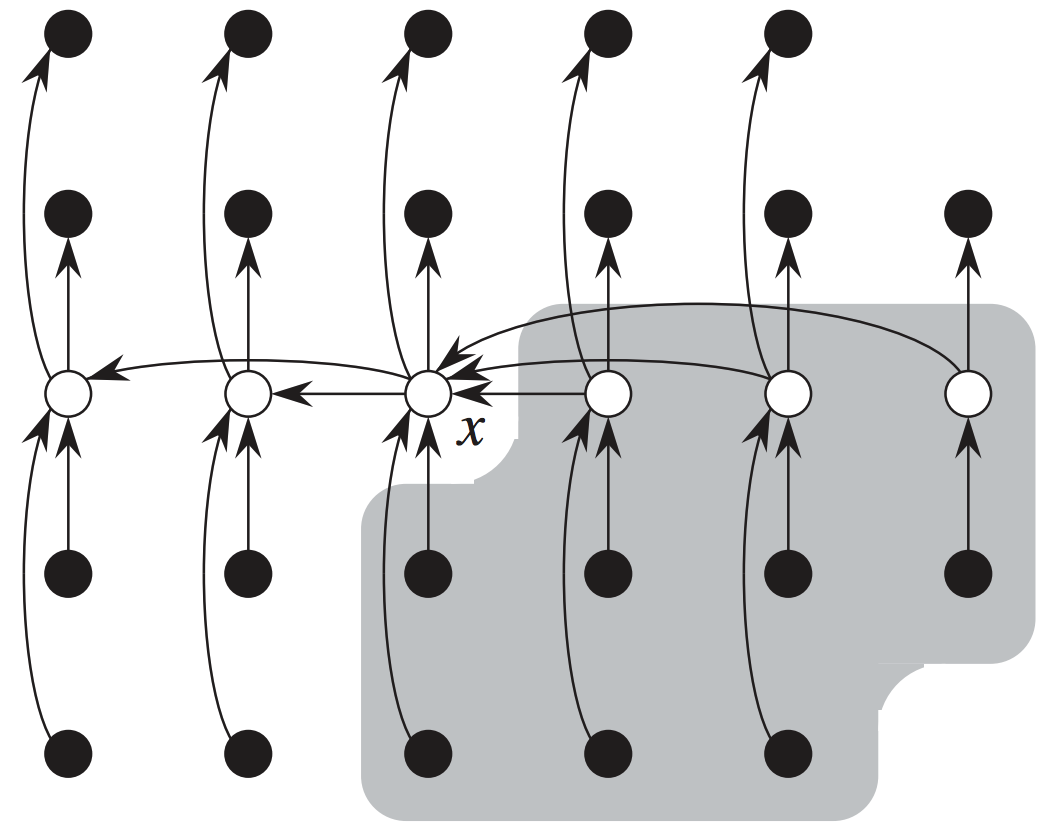
\includegraphics[scale=0.15]{median_of_medians.png}
\end{figure}

Half of the groups' medians must be less or equal to \( x \) by definition
of the median. For each of these groups, the median and the two elements
in the group less than the median are also less than or equal to \( x \),
contributing 3 elements per group.
\end{frame}

\begin{frame}
\frametitle{Runtime Analysis, continued}
\framesubtitle{}
There are \( \ceil{\frac{n}{5}} \) groups in total, but for simplicity we ignore
the group with \( x \) and the group with less than 5 elements,
so the number of elements less than \( x \)
is at least \( 3 (\ceil{\frac{1}{2} \ceil{\frac{n}{5}}} - 2) \)
or bounded below by \( \frac{3n}{10} - 6 \). \pause

Thus, in the worst case we recur on a list of size
\( n - (\frac{3n}{10} - 6) = \frac{7n}{10} + 6 \) \pause

This is basically a constant multiple!
Don't get too excited just yet, we added an additional recursive step because
\texttt{pivot} calls \texttt{select} to find the median
of a list of size \( \ceil{\frac{n}{5}} \).
\end{frame}

\begin{frame}
\frametitle{Runtime Analysis, continued}
\framesubtitle{}
First of all, we can decompose a list into groups of 5 and compute the
median of each group in linear time, since a sort of a list of size 5 is
\( O(1) \) and we perform \( \ceil{\frac{n}{5}} \) such sorts.
Thus, this median decomposition adds no asymptotic overhead
to the existing linear time partition step. \pause

If \( T(n) \) is the runtime of the algorithm on a list of size \( n \),
it fulfills the recurrence relation
\[ T(n) = O(n) + T(\ceil{\frac{n}{5}}) + T(\frac{7n}{10} + 6) \] \pause

Is \( T(n) \) \( O(n) \)? According to \textit{Introduction to Algorithms}, yes!

We can find the median of a list in linear time.
\end{frame}

\subsection{Decision Tree}

\begin{frame}
\frametitle{Decision Tree}
\framesubtitle{}
In practice, there's a large constant factor that could be optimized if we
could find the median of a list of size 5 quickly. \pause

We could model this problem as a \alert{decision tree}, where each internal node
contains a comparison, represented by two indexes to compare in the array,
i.e. \mintinline{python}{a[i] > a[j]}.
If the comparison is false, we recur on the left node
and if the comparison is true, we recur on the right node.
We continue until we reach a leaf node,
which simply contains the index of the median.
\end{frame}

\begin{frame}
\frametitle{Decision Tree, construction}
\framesubtitle{}
Suppose we build a decision tree to find the median of a particular list
containing \( n \) arbitrary and distinct elements. \pause

Claim: If the decision tree works on all \( n! \) permutations of this list,
then it works on \textit{any} list of \( n \) elements, even lists that contain
duplicate elements. \pause

Intuitively, we don't care about the actual values in the lists;
if the relative comparisons between the indexes are the same then we will
take the same path down the tree. \pause

Each set of \enquote{relative comparisons} defines an ordering of the list,
or a permutation. Thus, all lists have already been \enquote{covered}
by an corresponding permutation of our particular list. \pause

What about duplicate elements? \pause

I don't care how duplicate values compare to each other, because that just
determines the relative order of duplicates, which is arbitrary.
I can just pick any permutation that is correct for distinct value comparisons.
\end{frame}

\begin{frame}
\frametitle{Decision Tree, construction example}
\framesubtitle{}
The simplest particular list to pick is \( a = [0, 1, 2, 3, 4] \).
Suppose we have a decision tree which correctly identifies the median index
for each permutation of \( a \). \pause

Will this give the correct median for \( x = [0, 0.3, 0.2, 0.4, 0.1] \)?
Well, we can define the mapping \( 0 \rightarrow 0 \), \( 0.1 \rightarrow 1 \),
and so on. We know the decision tree works for \( [0, 3, 2, 4, 1] \),
a permutation of \( a \). Thus, it should work for \( x \). \pause

In general, we can construct this mapping by sorting the list and
mapping the value at \( x[0] \) to 0, \( x[1] \) to 1, and so on.
Thus, any list \( x \) has a corresponding permutation of \( a \)
with the same relative comparisons between any pair of indexes. \pause

If \( x \) has duplicate entries, then we can still apply the sorting algorithm
to generate a mapping. Of course, the corresponding permutation of \( a \)
\textit{won't} have the same relative comparisons, but this is acceptable
because relative comparisons between duplicate elements is arbitrary. 
\end{frame}

\begin{frame}
\frametitle{Decision Tree, properties}
\framesubtitle{}
There are two important properties of this decision tree:
\begin{enumerate}
  \item The height of the tree, which gives the number of comparisons in the
    worst case.
  \item The expected number of comparisons, assuming each permutation
    of the list occurs with equal probability. 
\end{enumerate} \pause
Of course, we want to minimize both height and expected number of comparisons.
How do we actually build such a decision tree?
\end{frame}

\begin{frame}
\frametitle{Decision Tree, construction}
\framesubtitle{}
Likely NP-hard in general, at least decision trees in a machine learning
context greedily maximize information gain at each level instead of trying
to globally optimize information gain. \pause

We could just generate every possible decision tree.
\( N = 5 \), how hard could it be?
Well, I have no clue because it takes at least 30 minutes,
at which point I terminated the program. \pause

We could prune trees by considering \textit{isomorphic} trees,
that is, we can take advantage of symmetry
(for example, the very first comparison is necessarily symmetric,
since there is no difference between any two pair of indexes). \pause

Instead, we'll use the greedy approach, and pick comparisons
that split the permutations between the left and right subtrees as evenly
as possible (very similar to kd-tree construction).
\end{frame}

\begin{frame}[fragile]
\frametitle{Decision Tree, application}
\framesubtitle{}
Once we have a decision tree, we can render it into Python.
\begin{minted}[label=median,fontsize=\tiny]{python}
def median(l: list) -> float:
    """ Computes the median of l, if len(l) == 5. """
    a, b, c, d, e = l
    return (((((((c if b < c else b) if b < d else d) if d < e else ((c if b < c else b) if b < e else e)) if c < e else (((e if b < e else b) if b < c else c) if a < e else (b if b < c else c))) if a < c else (((b if b < d else (d if a < d else a)) if b < e else ((d if a < d else a) if d < e else e)) if a < e else (a if a < d else ((e if d < e else d) if c < e else d)))) if c < d else (((((d if b < d else b) if b < c else c) if c < e else ((d if b < d else b) if b < e else e)) if d < e else (((e if b < e else b) if b < d else d) if a < e else ((b if b < d else d) if b < c else d))) if a < d else (((b if b < c else (c if a < c else a)) if b < e else ((c if a < c else a) if c < e else e)) if a < e else (a if a < c else (e if c < e else c))))) if a < b else (((((c if c < e else e) if a < c else a) if a < e else ((e if c < e else (a if a < c else c)) if b < e else ((a if a < c else c) if b < c else b))) if a < d else (((d if b < c else (d if b < d else b)) if a < e else (d if b < d else (b if b < e else e))) if d < e else ((e if b < e else (b if b < d else d)) if c < e else (c if b < c else (b if b < d else d))))) if c < d else ((((d if c < e else (d if d < e else e)) if a < d else a) if a < e else ((e if d < e else (a if a < d else d)) if b < e else ((a if a < d else d) if b < d else b))) if a < c else (((c if b < c else b) if a < e else (c if b < c else (b if b < e else e))) if c < e else ((e if b < e else (b if b < c else c)) if d < e else (d if b < d else (b if b < c else c)))))))
\end{minted}
\end{frame}

\begin{frame}[fragile]
\frametitle{Decision Tree, disappointment}
\framesubtitle{}
First, decision trees use on average 1.5 less comparisons than sorting,
and use at most 7 comparisons to find the median:
\begin{minted}[frame=none]{text}
Average value: 6.267, max depth: 7
Python sorted comparisions: 7.775
\end{minted}
According to \href{https://docs.python.org/3/library/timeit.html}{timeit},
decision trees win over sorting!
\begin{minted}[frame=none]{text}
ternary: 0.266674
   sort: 0.380404
\end{minted}
The difference is magnified with PyPy, about 26x faster:
\begin{minted}[frame=none]{text}
ternary: 0.002689
   sort: 0.070296
\end{minted}
In practice, however, decision trees are slower.
\end{frame}

\section{kd-Trees, Revisited}
\subsection{Nearest Neighbor Queries}

\begin{frame}
\frametitle{kd-Tree construction}
\framesubtitle{}
Back to kd-Trees. In order to use the linear time median algorithm derived
in the last section, we first generate a list of scalars from our list of points
by indexing each point at the current cutting dimension.

We then apply our median algorithm, and obtain a median \textit{value} in linear
time. Finally, we iterate through the points again, and pick any point with the
median value along the cutting dimension. \pause

Our construction complexity is now \( O(n \log n) \), since we avoid
the initial \( D \) sorts. Note how \( D \) does not appear in the complexity.
Claim: This complexity for (optimal) kd-tree
construction is asymptotically optimal.
\end{frame}

\begin{frame}
\frametitle{Nearest Neighbor}
\framesubtitle{}
\begin{block}{Nearest Neighbor Query}
  A \alert{nearest neighbor query} is given a point \( Q \) and a set of points
  \( P \), find the closest point to \( Q \) in \( P \). \pause
\end{block}
Suppose we build a kd-tree on \( P \). A kd-tree is helpful in the sense that
it gives us spatial data, as it successively partitions a space on hyperplanes
defined by points in the tree. \pause

We can take advantage of this by conducing a tree search,
with two important modifications:
\begin{enumerate}
  \item Keep track of the closest point so far, \( C \).
    Prune subtrees if they can't beat this closest point.
  \item Search subtrees in a order that maximizes pruning
\end{enumerate}
\end{frame}

\begin{frame}
\frametitle{Bounding Boxes}
\framesubtitle{}
Each subtree has a \alert{bounding box}, or the possible values it could take
on each dimension (i.e., a minimum and maximum value for each dimension).
If the distance between \( Q \) and the closest point in this bounding box
is greater than the distance between \( Q \) and \( C \), then there's
no point to search this subtree.
\begin{figure}[h!]
  \centering
  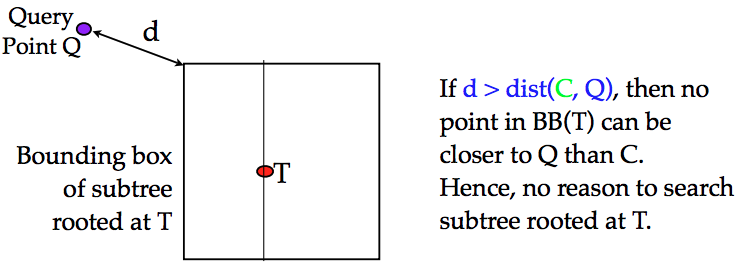
\includegraphics[scale=0.4]{nearest_neighbor_query.png}
  \caption{Justification for pruning subtrees}
\end{figure}
\end{frame}

\begin{frame}
\frametitle{Bounding Boxes, distance}
\framesubtitle{}
Question 1: How do we compute the distance between a point and a bounding box?
Let the bounding box be a list of tuples, each tuple being the minimum and
maximum value on that dimension.

\begin{exampleblock}{Bounding Box}
  The bounding box \( [(0, 5), (-2, 3)] \) defines a rectangle in the x-y plane,
  where \( x \) can be between 0 and 5 and \( y \) can be between -2 and 3.
\end{exampleblock}
\end{frame}

\begin{frame}
\frametitle{Bounding Boxes, distance}
\framesubtitle{}
As stated previously, the distance between a bounding box and a point \( Q \)
is the distance between \( Q \) and the closest point in the bounding box
to \( Q \). We can find this \enquote{closest point} by considering
each dimension separately, since in Euclidean distance each dimension
is independent of the others. \pause

Suppose we are on dimension \( d \). We have three cases to consider:
\begin{enumerate}
  \item \( Q[d] < bb[0] \), i.e. the point is left of the bounding box.
    In this case, we pick \( bb[0] \) along this dimension.
  \item \( bb[0] \leq Q[d] \leq bb[1] \), i.e. the point is in bounding box.
    We can just use \( Q[d] \) since it is contained.
  \item \( Q[d] > bb[1] \), i.e. the point is right of the bounding box.
    Similar to the first case, we use \( bb[1] \). 
\end{enumerate}

\end{frame}

\begin{frame}[fragile]
\frametitle{Bounding Box distance, code}
\framesubtitle{}
\begin{minted}[label=distance from a bounding box]{python}
  def distbb(p: tuple, bb: list) -> float:
      bbp = tuple(box[0] if x < box[0] else \
                 (box[1] if x > box[1] else x)
                  for x, box in zip(p, bb))
      return dist(p, bbp)
\end{minted}
\end{frame}

\begin{frame}
\frametitle{Bounding Boxes, computation}
\framesubtitle{}
Question 2: How do we keep track of these bounding boxes?
Well, we could say the initial bounding box at the root is completely unbounded,
i.e. \( (-\infty, \infty) \) on each dimension. When we traverse the
left and right subtrees, we must have split on some plane.

\begin{exampleblock}{Maintaining bounding boxes}
  Suppose we split on the value \( 5 \) along cutting dimension \( 1 \).
  Then for the left subtree we update \( bb[1] \) to be \( (-\infty, 5) \),
  and for the right we update \( bb[1] \) to be \( (5, \infty) \).
\end{exampleblock}

Note that these bounds are known \textit{a posteriori}, i.e. generated
online during the nearest neighbor search.
\end{frame}

\begin{frame}[fragile]
\frametitle{Bounding Box maintenance, code}
\framesubtitle{}
\begin{minted}[label=update bounding box,fontsize=\footnotesize]{python}
  def trimbb(bb: list, cd: int, p: int, d: int) -> list:
      if len(bb) == 0: return bb
      bb = list(list(box) for box in bb)
      bb[cd][1 - d] = p[cd]
      return bb
\end{minted}
\end{frame}

\begin{frame}
\frametitle{Subtree Order}
\framesubtitle{}
Lastly, we need to determine the order to search the subtrees.

It makes sense to first visit the subtree we would visit if we were inserting
the point in the kd-tree, i.e. the subtree which would contain the point.
\end{frame}

\begin{frame}[fragile]
\frametitle{Nearest Neighbor, code}
\framesubtitle{}
\begin{algorithm}[H]
  \caption{Nearest Neighbor Query}
  \begin{minted}[frame=none,fontsize=\scriptsize]{python}
    def __closest(self, t: "kdNode", p: tuple, bb: list) -> tuple:
        # bounding box too far away from point 
        if t is None or distbb(p, bb) > self.best_dist:
            return
        # update best point
        d = dist(p, t.point)
        if d < self.best_dist:
            self.best, self.best_dist = t.point, d
        # visit subtrees in order of distance from p
        i, j = t.dir(p), 1 - t.dir(p)
        self.__closest(t.child[i], p, trimbb(bb, t.cd, t.point, i))
        self.__closest(t.child[j], p, trimbb(bb, t.cd, t.point, j))

    def closest(self, p: tuple) -> tuple:
        self.best, self.best_dist = None, float("inf")
        bb = [[-float("inf"), float("inf")] for d in range(len(p))]
        self.__closest(self, p, [] if self.tight_bb else bb)
        return self.best
  \end{minted}
\end{algorithm}
\end{frame}

\begin{frame}
\frametitle{Runtime Analysis}
\framesubtitle{}
In the worst case, we need to traverse the entire tree, \( O(n) \).
In practice the runtime is closer to
\( O(\underbrace{2^d}_{\text{points in the neighborhood}} + 
\underbrace{\log n}_{\text{points \enquote{near} query}}) \)

If \( d \) is small, this is faster than \( O(nd) \) per query with the naive
method of searching every point. \pause

Note that we in fact introduce another \( d \) factor when we trim the bounding
boxes. However, the bounding boxes are the same regardless of the point we're
traversing the tree on, since the bounding boxes are a function of the tree
which doesn't change.
\end{frame}

\begin{frame}
\frametitle{Bounding Box, tight}
\framesubtitle{}
We can pre-compute bounding boxes, also taking advantage of \enquote{tighter}
boxes. The bounding boxes generated by the plane trim method generate boxes
that are too big - the real bounds are determined by the extrema of the 
\textit{points} contained in the subtree, not just the path to the subtree.
\pause
\end{frame}

\begin{frame}
\frametitle{Bounding Box, tight}
\framesubtitle{}
\begin{figure}[h!]
  \centering
  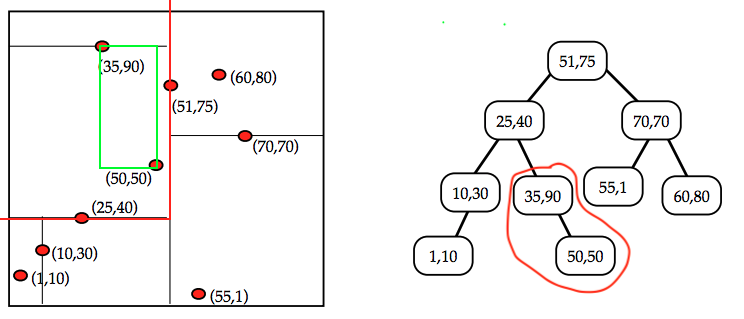
\includegraphics[scale=0.4]{bounding_boxes.png}
  \caption{Difference between the default (in red)
and tight bounding boxes (in green). Subtree is circled in red.}
\end{figure}
\end{frame}

\begin{frame}
\frametitle{Bounding Box, tight, computation}
\framesubtitle{}
The observation is that if we have a bounding box for both children of a node,
we can merge these efficiently since going up the tree means the bounding boxes
join together.

We have 3 cases:
\begin{enumerate}
  \item If we're a leaf, the only point we contain is the leaf's point.
    This serves as our bounding box (it just contains the point).
  \item If we have exactly one child, then we copy its bounding box and add
    the current node's point as well.
  \item If we have two children, we merge their bounding boxes and also add
    the current node's point. 
\end{enumerate}
\end{frame}

\begin{frame}[fragile]
\frametitle{Bounding Box, tight, code}
\framesubtitle{}
\begin{algorithm}[H]
  \caption{Tight bounding boxes}
  \begin{minted}[frame=none,fontsize=\scriptsize]{python}
    def tighten(self, t: "KdNode"=None) -> None:
        if t is None: t = self # called with None, set to the root 
        l, r, t.tight_bb = t.child[0], t.child[1], True
        # recur on children
        if l is not None: self.tighten(l)
        if r is not None: self.tighten(r)
        # leaf node, box is just the singular point
        if l is None and r is None:
            t.bb = [(t.point[d], t.point[d]) for d in range(t.D)]
        # one child, inherit box of child
        elif l is None or r is None:
            t.bb = l.bb if l is not None else r.bb
            # add node's point
            t.bb = [(min(box[0], v), max(box[1], v))
                    for box, v in zip(t.bb, t.point)]
        # two children, combine boxes
        else:
            t.bb = [(min(bbl[0], bbr[0], v), max(bbl[1], bbr[1], v))
                    for bbl, bbr, v in zip(l.bb, r.bb, t.point)]
  \end{minted}
\end{algorithm}
\end{frame}

\begin{frame}
\frametitle{Bounding Box, tight, runtime analysis}
\framesubtitle{}
After constructing a kd-tree, we can run \texttt{tighten} on the tree
to generate bounding boxes for each node.

\texttt{tighten} runs in \( O(ND) \) since we visit each node in the tree,
and at each node we do \( O(D) \) operations 
to do accounting on the bounding box. \pause

We assume that \( \log N > D \) or \( N > 2^D \), if \( D \) is very large
or \( N \) very small then kd-trees are not a good choice.
Thus, \texttt{tighten} is dominated by the \( O(N \log N) \) initial
construction time. \pause

We can run a nearest neighbor search as usual,
with the bounding box trimming logic removed.
\end{frame}

\begin{frame}[fragile]
\frametitle{Nearest Neighbor, code}
\framesubtitle{}
\begin{algorithm}[H]
  \caption{Nearest Neighbor Query with tight bounds}
  \begin{minted}[frame=none,fontsize=\scriptsize]{python}
    def __closest(self, t: "kdNode", p: tuple) -> tuple:
        # bounding box too far away from point 
        if t is None or distbb(p, t.bb) > self.best_dist:
            return
        # update best point
        d = dist(p, t.point)
        if d < self.best_dist:
            self.best, self.best_dist = t.point, d
        # visit subtrees in order of distance from p
        i, j = t.dir(p), 1 - t.dir(p)
        self.__closest(t.child[i], p)
        self.__closest(t.child[j], p)

    def closest(self, p: tuple) -> tuple:
        self.best, self.best_dist = None, float("inf")
        self.__closest(self, p)
        return self.best
  \end{minted}
\end{algorithm}
\end{frame}

\begin{frame}
\frametitle{Runtime Analysis}
\framesubtitle{}
First, we save the \( D \) factor because we no longer need to trim bounding
boxes, each node stores its boxes known \textit{a priori}. \pause

If we determine the bounding boxes based off the points in the tree,
then it is a subset of the original bounding box.
Thus, the distance between any point and our tight bounding box must be
greater than or equal to the distance between the point and the original
bounding box. We prune if the distance between the bounding box is greater
than the best distance, so our tight bounding box can only prune more
since it doesn't change the best distance found so far.

Pruning more means nearest neighbor searches run even faster.
\end{frame}

\begin{frame}
\frametitle{Wrapping it All Up}
\framesubtitle{}
We finally apply kd-trees to speeding up
\textit{k}-means/\textit{k}-means++.

Simply build a kd-tree on the centers,
re-building every time the centers change.
Whenever we need to find the closest center to a point, we do a nearest neighbor
query with the kd-tree. \pause

Per iteration, our running time is
\( O(\underbrace{K \log K}_{\text{kd-tree construction}} + 
\underbrace{N \log K}_{\text{\( N \) nearest-neighbor queries}}) \)

\( N \geq K \) so this is \( O(N \log K) \) per iteration, compared to
\( O(N K) \) for the naive algorithm. \pause

This is overly optimistic.
\begin{enumerate}
  \item Building a kd-tree naturally adds more memory consumption and overhead
  \item If \( D \) is very large, kd-trees become impractical
  \item kd-tree is \textit{expected} \( O(\log K) \), it could be \( O(K) \)
\end{enumerate}

TODO: Voronoi diagrams?
\end{frame}

\begin{frame}
\frametitle{Application of \textit{k}-means}
\framesubtitle{}
\begin{figure}[h!]
    \centering
    \begin{subfigure}[h]{0.3 \textwidth}
      
\includegraphics[scale=0.17]{hanekawa.png}
      \caption{Original image}
    \end{subfigure}
    \hfill
    \begin{subfigure}[h]{0.3 \textwidth}
      
\includegraphics[scale=0.17]{hanekawa8.png}
      \caption{\(k = 8 \)}
    \end{subfigure}
    \hfill
    \begin{subfigure}[h]{0.3 \textwidth}
      
\includegraphics[scale=0.17]{hanekawa256.png}
      \caption{\( k = 256 \)}
    \end{subfigure}
    \caption{\textit{k}-means on an image. Can you tell the difference
    at \( k = 256 \)?}
\end{figure}
The difference between naive and kd-trees gets larger as \( k \) increases.
For \( k = 8 \), kd-trees are roughly 2x slower, and for \( k = 256 \),
kd-trees are roughly 2x faster.
\end{frame}

\section{References}

\begin{frame}
\frametitle{References}
\framesubtitle{}
\begin{enumerate}
  \item Wikipedia articles on 
    \href{https://en.wikipedia.org/wiki/Color_quantization}{color quantization},
    \href{https://en.wikipedia.org/wiki/K-means_clustering}{\textit{k}-means},
    and \href{https://en.wikipedia.org/wiki/K-means\%2B\%2B}{\textit{k}-means++}
  \item \href{https://stanford.edu/~cpiech/cs221/handouts/kmeans.html}
    {Stanford \textit{k}-means handout}
  \item \href{https://www.cs.cmu.edu/~ckingsf/bioinfo-lectures/kdtrees.pdf}
    {CMU kd-Trees}
  \item \href{https://www.cs.cmu.edu/~ckingsf/bioinfo-lectures/kdrangenn.pdf}
    {CMU kd-Trees Continued}
  \item \href{https://mitpress.mit.edu/books/introduction-algorithms-third-edition}
    {\textit{Introduction to Algorithms}}, chapter 9
  \item \href{https://www.deviantart.com/ilikki/art/Shiny-Shaymin-Sky-498672972}
{Shiny Shaymin image}
  \item \href{https://pokemondb.net/artwork/shaymin}{Regular Shaymin image}
\end{enumerate}
\end{frame}

% \printbibliography
\end{document}
